
% #1 x, #2 y, #3 no, #4-6 text
\newcommand\nocswitchbuffertxt[6]{
    \draw (#1, #2) node[draw, thick, minimum width=2.5cm, minimum height=0.8cm, anchor=north, inner sep=0pt] (s1#3) {#6};
    \draw (#1, #2 + 0.8) node[draw, thick, minimum width=2.5cm, minimum height=0.8cm, anchor=north, inner sep=0pt] (s2#3) {#5};
    \draw (#1, #2 + 1.6) node[draw, thick, minimum width=2.5cm, minimum height=0.8cm, anchor=north, inner sep=0pt] (s3#3) {#4};
    \draw[thick] ([xshift=0.04em]s1#3.south west) -- ([xshift=0.04em, yshift=-1em]s1#3.south west);
    \draw[thick] ([xshift=-0.04em]s1#3.south east) -- ([xshift=-0.04em, yshift=-1em]s1#3.south east);
}

% #1 x, #2 y, #3 no, #4-6 text
\newcommand\nocnode[4]{
    \draw (#1,#2) node[draw, circle, thick, minimum size=1.1cm, inner sep=0pt] (#3) {#4};
}
% #1 x, #2 y, #3 no
\newcommand\nocnodestop[3]{
    \draw (#1,#2) node[draw, circle, thick, fill=black, minimum size=0.15cm, inner sep=0pt] (#3) {};
}

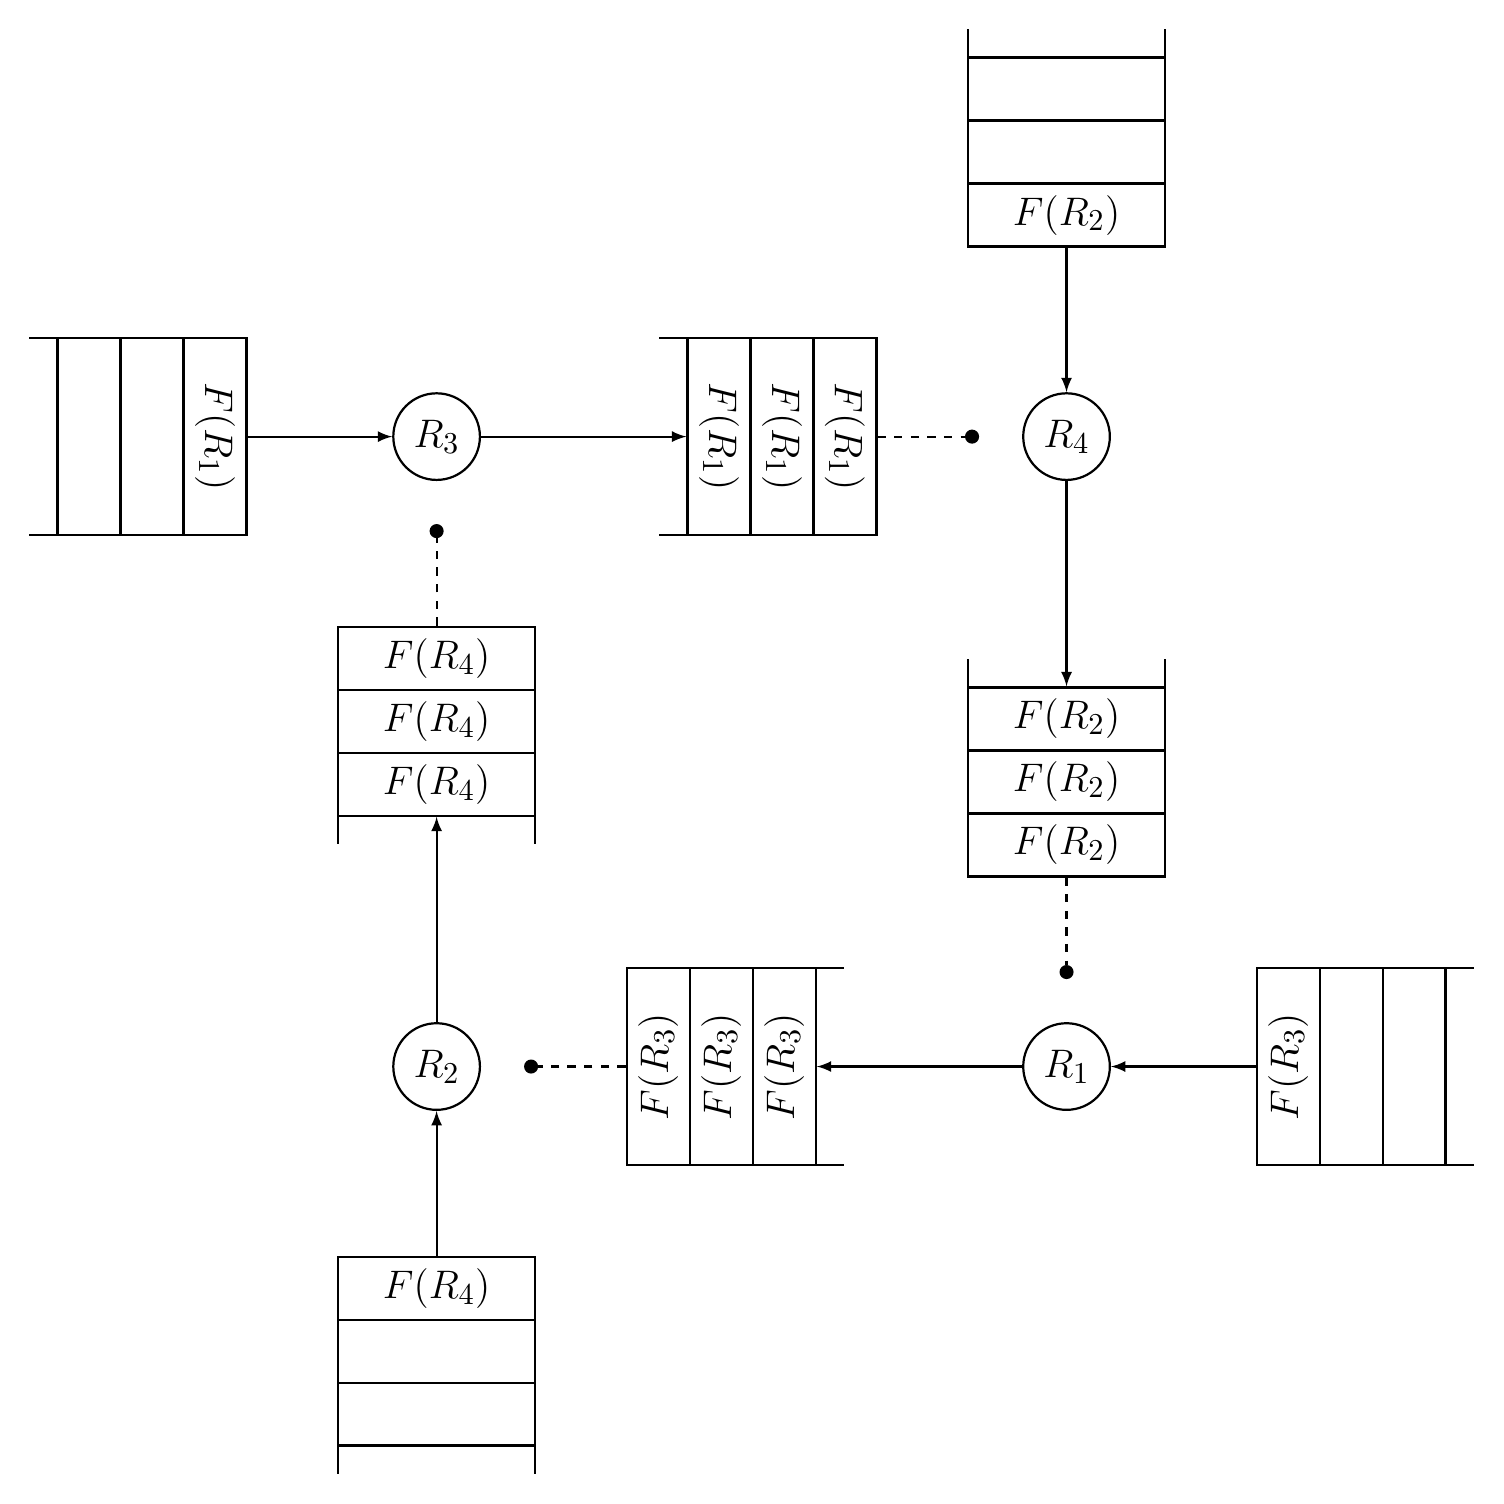
\begin{tikzpicture}[font={\fontsize{15pt}{12}\selectfont}]
\nocnode{0}{0}{r1}{$R_1$}
\nocnode{-8}{0}{r2}{$R_2$}
\nocnode{-8}{8}{r3}{$R_3$}
\nocnode{0}{8}{r4}{$R_4$}

\nocnodestop{0}{1.2}{stopr1}
\nocnodestop{-6.8}{0}{stopr2}
\nocnodestop{-8}{6.8}{stopr3}
\nocnodestop{-1.2}{8}{stopr4}

\nocswitchbuffertxt{-8}{-4}{sr2}{$F(R_4)$}{}{}
\nocswitchbuffertxt{-8}{4}{sr3}{$F(R_4)$}{$F(R_4)$}{$F(R_4)$}

\begin{scope}[rotate=-90, transform shape]
\nocswitchbuffertxt{-8}{-12}{wr3}{$F(R_1)$}{}{}
\nocswitchbuffertxt{-8}{-4}{wr4}{$F(R_1)$}{$F(R_1)$}{$F(R_1)$}
\end{scope}

\begin{scope}[rotate=90, transform shape]
\nocswitchbuffertxt{0}{-4}{er1}{$F(R_3)$}{}{}
\nocswitchbuffertxt{0}{4}{er2}{$F(R_3)$}{$F(R_3)$}{$F(R_3)$}
\end{scope}

\begin{scope}[rotate=180, transform shape]
\nocswitchbuffertxt{0}{-12}{nr4}{\rotatebox{180}{$F(R_2)$}}{}{}
\nocswitchbuffertxt{0}{-4}{nr1}{\rotatebox{180}{$F(R_2)$}}{\rotatebox{180}{$F(R_2)$}}{\rotatebox{180}{$F(R_2)$}}
\end{scope}


\draw[thick, ->, >=latex] (s3sr2.north) -- (r2.south); 
\draw[thick, ->, >=latex] (s3wr3.north) -- (r3.west); 
\draw[thick, ->, >=latex] (s3nr4.north) -- (r4.north); 
\draw[thick, ->, >=latex] (s3er1.north) -- (r1.east); 

\draw[thick, ->, >=latex] (r2.north) -- (s1sr3.south); 
\draw[thick, ->, >=latex] (r3.east) -- (s1wr4.south); 
\draw[thick, ->, >=latex] (r4.south) -- (s1nr1.south); 
\draw[thick, ->, >=latex] (r1.west) -- (s1er2.south); 

\draw[thick, dashed] (s3nr1.north) -- (stopr1); 
\draw[thick, dashed] (s3er2.north) -- (stopr2); 
\draw[thick, dashed] (s3sr3.north) -- (stopr3); 
\draw[thick, dashed] (s3wr4.north) -- (stopr4); 

 
\end{tikzpicture}
